\chapter{System Design}
\label{ch:design}
\acresetall

This chapter portrays the design for the proposed implementation of the secure
ad hoc network. The design here is based on a functional pro-active ad hoc
routing protocol. The routing is left to the chosen routing protocol, i.e.
\ac{BATMAN}, and the changes made will not affect how the routing is performed.
The system design is an extension of the protocol, which requires nodes to be
authenticated and trusted before being allowed into the network. To strengthen
the system each node also has to verify its identity periodically, or it is
dropped from the network.

\section{Brief Overview}
In this section a short version of the system design is described. It is far
from complete when it comes to explaining the entities, messages being sent,
system states, and why certain choices have been made. This section is
suggested to read through in its entirety just in order to get an overview of
what the system does, leaving the explanations to the subsequent sections.

\subsection{Initial Authentication}
The network setup starts with an out-of-band authentication where a master node,
hereafter \ac{SP}, verifies new nodes. How this is done can be up to the
application, but let us assume that the actors carrying their communication
devices, hereafter nodes, physically meet the \ac{SP} at the scene and verify
each others' public keys out-of-band.

When a new node is discovered by the \ac{SP} using regular routing announcements
as part of the pro-active routing protocol, the \ac{SP} will invite the new node
to a handshake to establish a trust relationship between the two nodes. In the
invite message the \ac{SP} shares its certificate. If the node can verify the
public key of that certificate, it will request a proxy certificate. If the
\ac{SP} can verify the new node's public key, too, it will issue a proxy
certificate with (possibly) the rights to participate in building the
\ac{MANET} by broadcasting its own and re-broadcasting other trusted nodes'
routing announcements. Note that the routing announcements of the new node will
not have been forwarded by other nodes up until this point, and therefore the
new node and the \ac{SP} would have had to be direct neighbors throughout this
handshake.

\subsection{Continuous Authentication}
After being issued with a \ac{PC} the newly authenticated node will periodically
``broadcast'' - unicast to each neighbor - a message containing an ephemeral key
and corresponding \ac{IV}, a pseudo-randomly generated nonce, and a digital
signature over this message. The ephemeral key is encrypted with the neighbor's
public key (hence multiple unicasts instead of an actual broadcast), but the
digital signature is generated using the hash of the unencrypted key and the
other contents of the message. If you at this point want to see how this
keystream generation works, you can jump to Figure
\ref{fig:keystream_generation}.

After sending this signed ``broadcast" to each neighbor, the node and its
neighbors will generate a keystream from the ephemeral key, \ac{IV}, and nonce.
The node will then append two new bytes from this keystream to each routing
announcement, and re-broadcasts of neighbors announcements, sent from this point
forward with a sequence number for the recipient to be able to match this
``extract'' with the keystream at an offset given by the sequence number.

TODO: FIGURE SHOWING KEYSTREAM-MATERIAL PACKET, JUST PACKET NOT MSC

The neighbors accepts a routing announcement if and only if:

\begin{itemize}
  \item the routing announcement is appended with a key extract and,
  \item it matches the sender's keystream at the sequence number offset and,
  \item that sender's sequence number has not been received earlier (replay).
\end{itemize}

This ``key extract'' of the keystream is comparable to regular \acp{OTP} as used
by e.g. online banks and it is important to note that they are not ``connected''
to the routing announcements sent, meaning they do not provide integrity for the
packet.

Note also that each node has its own keystream, and that it shares the message
above, hereafter ``keystream-material message'', with each of its direct
neighbors. Each neighbor then use this node's keystream to verify its routing
announcements.

Whenever a routing announcement is forwarded by another trusted node, that
node will replace the one-time password with an \ac{OTP} from its own keystream.
This way every node only checks its direct neighbor for authentication, which is
a design choice. This proposal assumes that because every node is verified by
the \ac{SP} in the first place, all nodes in the network will be able to trust
each other, which also means they will trust their neighbors to properly verify
their neighbors again. This technique also helps prevent a wormhole attack,
which will be discussed later.

%In order for trusted nodes to learn of newly trusted nodes existence, the
%\ac{SP} reularly broadcasts lists containing the id, address and public key of
%each trusted node in the network. This needs to be done, because before
%learning about a new node the other trusted nodes will not accept any messages
%from this node. This means the new node will not be able to exchange its own
%\ac{PC} with other nodes directly - only through the \ac{SP}.

When a trusted node discovers a new neighbor, which is a trusted node in the
network, they first have to exchange their \acp{PC} and verify the signatures
on the certificates. Their knowledge of the corresponding private keys to their
\acp{PC} are verified later when they check each other's digital signatures on
the keystream-material messages. Also, without the knowledge of the private key
they would not be able to decrypt the ephemeral keys received in the same
packets. Each of the two nodes then stores the other's public key, subject name,
id, role, and address in a list called \ac{AL}.

%The list, hereafter \ac{AL}, also adds some \ac{WOT} like capabilities. The
%list is signed by the \ac{SP}, which means the integrity of the list is
%guaranteed by the \ac{SP}. This means that if the \ac{SP} should go offline,
%e.g. it could be out of range, other trusted nodes in the \ac{MANET} can
%continue to broadcast the \ac{SP} on behalf of the \ac{SP} - to ensure all
%nodes in the network know each other. This can be especially important when the
%network grows large and become fully or partially separated and nodes in one
%part may not have learnt of the existence of newly trusted nodes yet. It also
%applies to trusted nodes who have been offline while new nodes have been
%verified, then re-enter the network while the \ac{SP} is offline. [TODO:
%kanskje ref til mitt eget essay?]

After a neighbor is added to the \ac{AL}, the node can then also add the
neighbor to another list, called a \ac{NL}. This list is used to keep
track of current direct neighbors and their current keystreams. While nodes in
the \ac{AL} are kept in that list throughout the lifetime of the network, or
until the lifetimes of the nodes' certificates have expired, a node in the
\ac{NL} is removed when it is no longer a direct neighbor. 

\section{Requirements}
Ad hoc networks have some desired characteristics such as quick and inexpensive
setup and being independent of communication infrastructure, but they also
impose great challenges regarding security. The challenges regarding security
can vary depending the purpose and environment of the network which will be
covered in this section.

\subsection{Scenario}
The design and implementation presented in this thesis is mostly based on an
emergency situation scenario, in which a communication infrastructure is
unavailable. This thesis will also reflect on some possible requirements given
by a military application.

If there is a major emergency situation such as an earthquake or tsunami, it is
likely that parts or the entire communication infrastructure at the scene
is destroyed or temporarily down. The remaining communication lines will then
probably be congested, such that little communication actually goes through.

In this situation, it is of great importance that Emergency Personnel, such as
Paramedics, Firemen, Policemen and the Military, are able to communicate
efficiently and therefore independently of the public communication
infrastructure. They need this network in order to manage the the operation, and
therefore availability is probably the most important trait of this network.
Secondly, they should be able to trust the communication on the network - i.e.
messages sent are from whom they claim they to be.

Also, being able to authorize new actors on the scene, such as Red Cross, can be
critical to the operation. These new actors will probably not have the necessary
authentication tokens, i.e. certificates, required by the authentication scheme
in the network.

\subsection{List of Requirements}
Based on the scenario above these requirements can be extracted and made into
general requirements that needs to be addressed by the system design. The work
presented here is based on several sources, most prevalent being the research
from the OASIS project \cite{oasis_report} \cite{5683058} \cite{nyre2009secure}
and the doctoral project of Eli Winjum carried out at UniK
\cite{ffi_2005_04015}.

\begin{table}[ht!]
	\centering
	%\begin{tabular}{ | l | p{11cm} | }
	\begin{tabular*}{\textwidth}{ | p{5mm} | p{388pt} | }
	\hline
	\textbf{\#} & \textbf{Requirement Description}\\\hline
		R1 & A node must be authorized in order to get full rights in a network \cite{dahill2001secure}, \cite{sanzgiri2002secure}\\\hline
		R2 & A node without a recognized authentication token should be able to become authorized if necessary\\\hline
		R3 & Networks need a master node to handle authentication of new nodes\\\hline
		R4 & Access control (after initial authentication) should work without centralized nodes\\\hline
		R5 & Different networks should be able to collaborate \cite{ffi_2005_04015}\\\hline
		R6 & Only master nodes can decide access policies of users/nodes\\\hline
		R7 & Nodes must not be able to alter their access policies\\\hline
	\end{tabular*}
	\caption{Requirements based upon our simplified and general scenario.}
	\label{tab:our_req}
\end{table}

An early study produced security requirements of ad hoc networks demanding
that the routing logic must not be spoofed or altered to produce different
behavior \cite{dahill2001secure}. R1 is constructed from that requirement.
During the OASIS project, a requirement ensuring different actors such as
police, fire and medical professionals can participate in the network, gives R2
\cite{5683058}.

Because of R2 there needs to be some sort of authority managing the
authentication and access management, which leads to R3. However, verifying
nodes access rights after the fact should be possible even without the
availability (R4) - also a requirement given by the OASIS project.

The doctoral project of Winjum recommends seamless radio coverage over the whole
crisis area, possibly requiring merging or at least collaboration between
different networks, R5.

R7 comes implicitly from R6 because R6 would be useless if regular nodes could
alter their priveleges without the permission of a master or management node. R6
is necessary in this design as no authentication is required prior to the
network setup, and it is therefore no way to know which rights one actor/node
shuold have. As will be discussed in Chapter \ref{ch:discussion} the network
might also be able to recognize authentication tokens, such as long lived
certificates, issued prior to this setup. If this is the case, one might have to
re-evaluate these requirements.

The OASIS project had another important requirement which is not covered here,
but is important to mention - there should be mechanisms in place to detect
misbehaving nodes, i.e. already trusted nodes that act maliciously. This
detection is not covered in this thesis as pointed out in
\ref{limit:malicious_behaviour}, but is nevertheless important to take notice
of.

\section{Why use Proxy Certificates?}
\acp{PC}, as described in Section \ref{sect:pc}, are used to delegate
rights on behalf of their issuers. That means that the issuer, i.e. the \ac{SP},
can choose to delegate all or a subset of its rights to the receiver of the
\ac{PC}. This can be very useful in a situation where the nodes themselves are
unable to properly authenticate themselves with their pre-existing \acp{LLPKC}
if the \ac{SP} on the scene has no way to verify their certificates. This can be
true if their certificates are issued by an unknown root certificate (\ac{CA})
or simply if there is no Internet access and the certificate is signed by an
unknown entity (unknown to the \ac{SP}), even if it knows and trusts the root
\ac{CA}. 

In addition, proxy certificates commonly have a short valid lifetime compared to
regular certificates, meaning an implementation using proxy certificates does
not necessarily need to implement a certificate revocation scheme, which makes
for less management operations in the management-hostile environment that is
\acp{MANET}. If a certificate is compromised in this \ac{MANET}, the time of
exposure is limited because of the short valid lifetimes on the \acp{PC}.
Regular \acp{LLPKC} on the other hand, could be compromised throughout the
lifetime of the network, or until revocation lists were brought to the scene,
out-of-band or by acheiving Internet access later on.

Also, the \ac{SP} could be interested in giving the node rights the node would
not usually have on this specific scene, depending on the situation. This is
easier to achieve when the \ac{SP} can delegate its own rights. Different nodes
can be given different rights, as long as they are a subset of the SP's rights.
There are countless of different potential rights that can be useful for a
network, given the situation they are used in, and here is a few possible
rights/privileges to give the reader an understanding of the possibilities they
give:

\begin{itemize}
  \item Announce itself - let the \ac{MANET} know of your existence
  \item Re-broadcast other nodes' announcements - reshape the network topology
  \item Announce a gateway - give the \ac{MANET} access to another network
  \item Use the gateway - allow you to communicate outside the \ac{MANET}
  \item Send and receive messages with a defined application - full application
  rights
  \item Only receive messages from a defined application - limited application
  rights
\end{itemize}

The different choices are essentially up to the \ac{SP} managing the network.
One can ask why this is necessary, and again it depends on the application. If
you are setting up a \ac{MANET} on the scene of a disaster to assist emergency
personnel, you could have some actors be able to organize the effort by sending
orders/commands to the other actors, while some actors only are allowed to
receive the orders. In this situation it might be of great importance to know
that only verified nodes are able to give commands, but the importance of
getting this information available outweighs the need to verify the nodes/actors
receiving this information.


\section{Design Overview}
The secure ad hoc network designed here does not change any fundamental workings
of regular ad hoc routing protocols. When nodes have been authenticated and
neighbors have verified their neighbors respectively, the routing annoucements
are generated, broadcasted, forwarded, and handled by the routing protocol
almost as usual. The only addition to the routing protocol is the addition of
one-time passwords (OTP) to the routing announcements, and the handling of said
\acp{OTP}.

The proposed design should work with most pro-active ad hoc routing protocols
operating on the network layer with limited alterations - but this design is
specifically made for the BATMAN \cite{batman_rfc} routing protocol chosen for
its simpler design compared to e.g. OLSR \cite{clausen2003rfc3626} and because
it operates on the third layer of the \ac{OSI} model \cite{zimmermann1980osi}.
Whether this design would work on a link-layer protocol is unknown, and there is
still a discussion whether having routing protocols on the link-layer is a good
thing, as it breaks the layering principles of the \ac{OSI} model
\cite{5680190}. How this design is incorporated, or added, to the BATMAN
protocol will be explained in Chapter \ref{ch:implementation}.

The basic principle of the proposed design is that an authenticated node accepts
other authenticated nodes' routing announcements and forwards them as normal, while
discarding routing announcements from unauthenticated nodes. One or more nodes in the
network will assume a role as master node(s), or a \ac{SP}, with the extra
capability of authorizing new nodes into the network. A special certificate
called a \ac{PC} \cite{rfc3820} will be used for authentication after this
authorization has taken place such that other nodes in the network will be able
to authenticate and accept the new node.

\subsection{Entity Explanation}
Before a simplified example can be given, a few new entities in this design
needs to be explained further. This is the short version, just enough for the
reader to understand the example - the full description of these entities
and why they are necessary will be given in Section \ref{sect:detailed_ent}. All
of these entities are also portrayed in Figure
\ref{fig:simple_example_entities}. The portrayed entities will be used as a
template for other figures later in this thesis report.

\begin{itemize}
  \item \textbf{\acf{SP}} is responsible for tasks similar to that of a \ac{CA}
  	and has the master role in the network. The \ac{SP} is the entity that
 	authorizes new nodes and signs their \acp{PC}.
  \item \textbf{\acf{PC0}} is a \ac{PC} belonging to a \ac{SP} signed by its
    regular \ac{LLPKC}. This \ac{PC} has a certificate depth of 0, thus we refer
    to it as a \ac{PC0}.
  \item \textbf{\acf{PC1}} is a \ac{PC} signed by a \ac{PC0} (i.e. by the
    private key of the \ac{SP}). All authenticated nodes in one network, has at
    least a \ac{PC1} signed by a \ac{SP} from that network.
  \item \textbf{\acf{AL}} is a list containing the necessary information about
 	all known and authorized nodes in the network. All nodes keep a local copy of
 	the \ac{AL} which they use to authenticate other nodes in the network.
  \item \textbf{\acf{NL}} is a list containing the current trusted direct
    neighbors with a copy of their keystreams used for verifying their routing
    announcements. The \ac{NL} is a subset of the \ac{AL} and a node must be
    found in the \ac{AL} before it can be added to the \ac{NL}.
  \item \textbf{Authenticated/Trusted Node} is a node which has been issued a
    \ac{PC1} from the \ac{SP} and is considered a trusted node in the network.
    This node can take part in sending its own routing announcements and
    forwarding other authenticated nodes' routing announcements, i.e. they take
    part in changing the network topology.
  \item \textbf{Unauthenticated Node} is a node which has not yet been
    authorized, or denied access, by the \ac{SP}. It does not possess a
    certificate for which the other nodes can verify, and its routing
    announcements are ignored by other trusted nodes in the network.
\end{itemize}

\begin{figure}[h]
	\centering
  	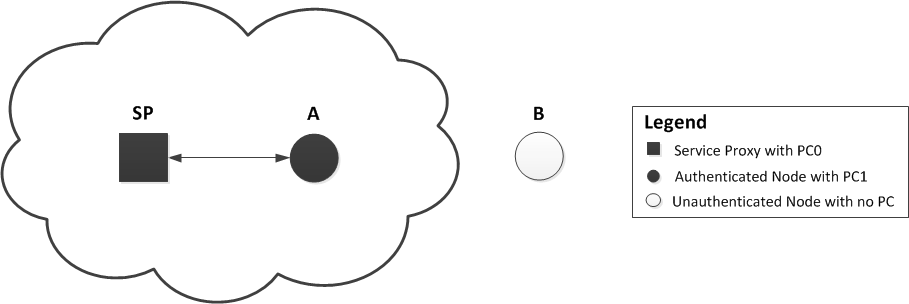
\includegraphics[width=\textwidth]{images/simple_example_entities.png}
  	\caption{Different entities in the Simple Example.}
	\label{fig:simple_example_entities}
\end{figure}

\subsection{Simple Example}
Two nodes are within transmitting range of each other, i.e. they are direct
neighbors. One of the nodes is a \ac{SP} and the other is unauthenticated. The
pro-active ad hoc routing protocol used on both nodes regularly broadcasts
routing announcements, so the two nodes learn of each others' existence - i.e.
they ``discover'' each other. Upon reception of a routing announcement from the
unauthenticated node, the \ac{SP} will invite the node for a handshake. The
invite message contains the \ac{SP}'s \ac{PC0} which assumably the
unauthenticated node is able to verify, possibly based on a prior out-of-band
sharing of public key fingerprints.

After verifying the \ac{PC0}, the unauthenticated node will send a \ac{PC}
request with its own public key. If the \ac{SP} is able to verify the sender's
public key (same assumption as above) and the \ac{SP} decides this node should
have access to network, it will create and sign a \ac{PC} for this node - i.e.
the node is issued a \ac{PC1}.

%Before the \ac{SP} actually signs the \ac{PC} requested from the
%unauthenticated node, it needs some verification that the node is an actor that
%should be allowed access to the network. The actor will therefore meet the
%\ac{SP} in the field and give its public key fingerprint (out-of-band) so the
%\ac{SP} can verify the incoming public key in the \ac{PC} request as the
%actor's request.

%Using the public key of the \ac{PC1}, the newly trusted node will now create
%and broadcast a signature, and use an excerpt (offset value) from this
%signature in its routing announcements. The signature excerpt is just a value used
%in the following routing announcements, and not the cryptographic signature itself,
%but will be used for recognition. This will be described further later in the
%chapter. The \ac{SP}, recognizing the signature offset value will rebroadcast
%the routing announcements so regular ad hoc routing follows.

When the handshake completes both nodes will add the other node of the handshake
to their \ac{AL} - storing their id, address, unique subject name, role, and
public key. All the steps up to this point is portrayed in the first half of
Figure \ref{fig:simple_example_msc}. As illustrated by the color of the node
circle, the new node (A in the figure) is authenticated after receiving the
issued \ac{PC1}.

Next, both the newly authenticated/trusted node and the \ac{SP} will send one
another a packet called a ``keystream-material message" containing their
current (or new in the case of the trusted node) ephemeral key, \ac{IV}, nonce
value and a digital signature over the hash of these values. Before sending
this message, the ephemeral key part is encrypted with the other's public key
to keep this information secret. Note that the digital signature however, is
computed over the unencrypted key in order to re-use this signature for all
neighbors the node has to send this message to.

Both nodes can now generate the other's keystream (and the new node its own),
hence the name ``keystream-material message'', used to verify the sender of
subsequent routing announcements. These keystreams, address, id, an empty ``last
sequence number'', and an empty sliding window of the other node is then stored
in the \ac{NL}.

%Also upon handshake completion is the generation an \ac{AL}. The \ac{SP} will
%use this list in order to save certain necessary details about the other node,
%such as its address, public key, last signature, and more. Also in this list is
%the corresponding information about the \ac{SP} itself. When the list is
%created or updated it is broadcasted to the network - signed by the \ac{SP} to
%ensure no other node can alter the information about trusted nodes in the
%network.

From this point forward, the two nodes use a two-byte extract of the keystream
as an one-time password and appends it, together with a sequence number (for
finding the correct offset in the keystream), to future routing announcements.
This goes for both original routing announcements from the node itself, and when
they forward other trusted nodes' routing announcements. The two nodes never
re-use the same extract from the keystream, hence the name ``\acf{OTP}'', and
they use a sliding window stored in their \ac{NL} to keep track of which
extracts they have received from their neighbor. This last part is crucial in
order to be able to drop announcements containing re-used extracts, avoiding
replay attacks. 

Whenever a new node is discovered by the \ac{SP} the procedure above repeats,
and a new addition is made to the \ac{AL} and \ac{NL}. Other previously
trusted nodes will learn the identity of new nodes when they discover the new
node and initiate a keystream-material exchange, which will be discussed
later.

\begin{figure}[ht]
	\centering
  	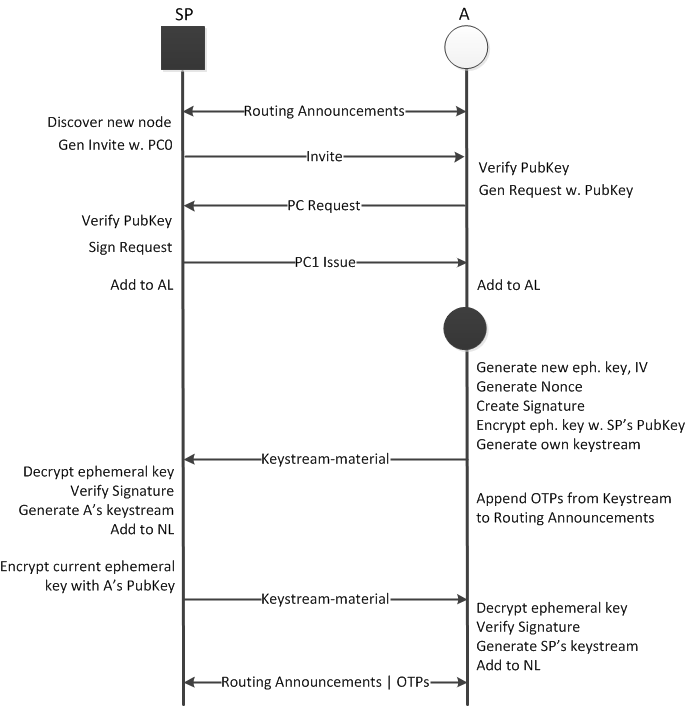
\includegraphics[height=13cm]{images/simple_example_msc.png}
  	\caption{Authentication handshake and keystream-material between a new node A and the SP.}
	\label{fig:simple_example_msc}
\end{figure}

Figure \ref{fig:simple_example_msc} shows a message sequence chart of the
messages sent between two nodes during the simple example. The second
half portrays the messages sent in a keystream-material message and that
they are added to the \ac{NL} after these have been received, and after
the \ac{AL}-addition. Routing announcements without \aclp{OTP} are sent
periodically throughout the sequence until keystreams are generated, but this
is left out of the figure as they do not affect the nodes. Only the routing
announcements in the beginning and in the end that are appended with \acp{OTP}
are portrayed as they show how the handshake is initiated (by discovery) and
ended after successfully ending the handshake and keystream material sharing.

If a new node enters transmitting range of the two nodes, similar messages are
exchanged, as shown in Figure \ref{fig:simple_example_msc_2}.

\begin{figure}[h]
	\centering
  	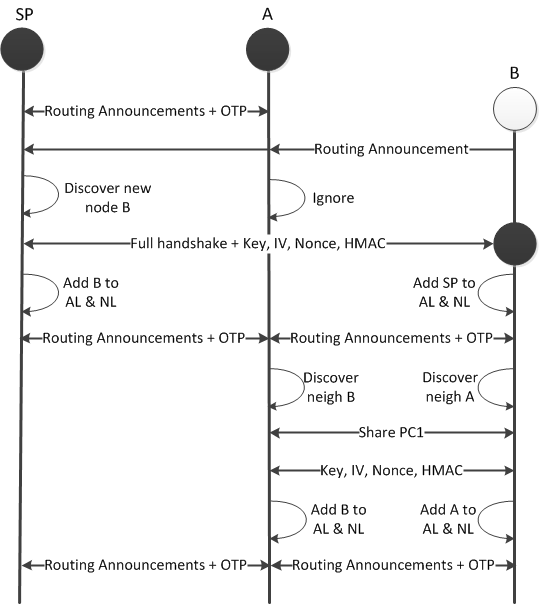
\includegraphics[height=13cm]{images/simple_example_msc_2.png}
  	\caption{Another node B joins the network from previous figure.}
	\label{fig:simple_example_msc_2}
\end{figure}

Here we see that after node B has been fully authenticated and started
broadcasting routing announcements appended with its own \acp{OTP}, he and node
A will ``discover'' each other. Up until this point node A has ignored node B's
routing announcements (and forwarded announcements) because they have not been
appended with any valid/recognizable \acp{OTP}.

After they've discovered each other they share their certificates as seen in the
figure. Before continuing they need to verify each other's certificate, which is
to verify the signature on the \ac{PC1}'s up against the public key of the
\ac{SP}.

When both nodes have verified each other's certificates, they send each other
their keystream-material messages, in which they verify each others' signatures
to actually verify each other as the legitemate owners of the certificates. If
they are able to verify each others' signature they will add each other to their
\ac{AL} and \ac{NL}, respectively.

\section{Authentication Phase}
This section is devoted to explain the phases a node goes through before and
when authenticating itself to the network. These phases should be similar for
most network layer pro-active routing protocols as the main trigger of these
phases are the routing announcements sent as per normal operation of any
pro-active routing protocol.

\subsection{Node Discovery}
Upon entering the network area, the node is both unauthenticated and unknown to
the network. Because it uses a pro-active routing protocol, the node regularly
broadcasts routing announcements to be received by any potential node in the
area. At this point an assumption that all nodes are configured with unique
addresses and with the same netmask is done in order to focus on the security
challenges, rather the non-trivial task of assigning addresses in \acp{MANET}
(See Limitations in Section \ref{limit:ip_address_conf}). With this assumption all
nodes within transmitting range of the new node can receive its broadcasts.

\begin{figure}[h]
	\centering
  	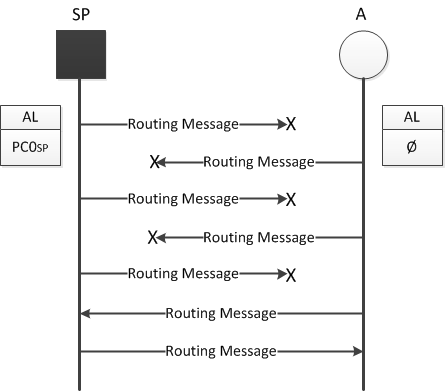
\includegraphics[width=0.6\textwidth]{images/node_states_discovery.png}
  	\caption{Discovery Phase between a SP and an unauthenticated node A.}
	\label{fig:node_states_discovery}
\end{figure}

Simultaneously, the node also listens to other nodes' routing announcements.
Depending on the time interval between the broadcasts and whether the nodes
within each other's transmitting range are asymmetrical, they will discover each
other approximately at the same time.

Figure \ref{fig:node_states_discovery} illustrates the routing announcements
periodically sent by two nodes until they discover each other. One of the nodes
have already assumed the master role and is a \ac{SP} while the other node is
unauthenticated.

The \ac{SP} will have a \ac{PC0} and its \ac{AL} has only one entry - itself.
Note that if it had authorized another node at an earlier point in time (but
within the lifetime of the \ac{PC}) that node's values would also be
represented in the \ac{AL}, even if the node was outside the network at this
point in time (physically).

The new node does not have any \ac{PC} at this point, unless it has a \ac{PC}
issued within and valid only for another network. This is however not covered
here, and it is assumed the node has no certificate at all. The same goes for
its \ac{AL}, or one can rather say it has an empty \ac{AL} - denoted by the
'\O' in the figure.

\subsection{Authentication Handshake}

\begin{figure}[h]
	\centering
  	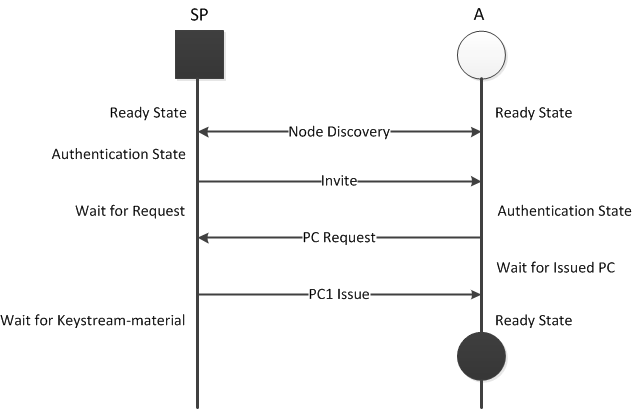
\includegraphics[width=0.6\textwidth]{images/node_states_handshake.png}
  	\caption{Handshake between a \acf{SP} and an unauthenticated node A.}
	\label{fig:node_states_handshake}
\end{figure}

Once the two nodes have discovered each other, the \ac{SP} will enter an
authentication handshake state, while the unauthenticated node will not do
anything. The authentication handshake state of the \ac{SP}, and later of the
other node, does not obstruct regular routing announcements to be sent. The
current state only affects how the \ac{AM} operates, not how the original
routing protocol operates. Actually, the handshake and all other messages and
operations handled by the \ac{AM} is executed in a separate thread and sent
and received using another socket than the rest of the protocol. This is
further elaborated in the next chapter.

Because the unauthenticated node does not enter a new state upon the discovery
of the \ac{SP}, which could just be a regular authenticated node as well, there
will be no deadlock if for some reason the \ac{SP} should never initiate, or
invite to, the handshake. This could happen for a multitude of reasons where
the two nodes lose their connectivity between each other because of the flaky
nature of wireless ad hoc networks, or the assumed \ac{SP} was only a regular
authenticated, trusted, node. From the routing announcements it is not possible
to derive whether a node is simply authenticated, or if it also has master role
capabilities being a \ac{SP}. It is only possible to derive, or rather it seems,
that a node is authenticated in some network or not.

%The unknown node will wait for a predefined amount of time, for it may not ever
%receive a request. The discovery might have been of an authenticated node with
%a \ac{PC1} and not a \ac{SP}, which does not have the rights to authenticate
%new nodes. It might also have been that of a \ac{SP}, but because of the flaky
%nature of ad hoc networks, the two nodes might have become invisible to each
%other before the handshake could be initiated.

While the new node is ``waiting'' for an invite, or simply not doing anything
other than announcing its existence - the \ac{SP} generates an invite message
which is a message containing its \ac{PC0}. The invite will be directly
addressed to the new node, and not broadcasted as regular routing announcements
are. The \ac{SP} will then wait for a certificate request (\ac{PC} Request) for
a short predefined time before aborting the handshake and entering its
ready-state. If the two nodes discover each other once more, the \ac{SP} will
once again try to invite the other node to the handshake. If this fails several
times, the \ac{SP} will eventually ignore all the discoveries of the other node
(based on address) for a predefined time before it tries again.

If the new node is able to verify the SP's public key it will use its public
key pair and generate a \ac{PC} request which it will send back to the \ac{SP}.
This request abides by the rules for making a proxy certificate \cite{rfc3820},
setting the ``Issuer Name'' the same as the ``Subject Name'' from the received
\ac{PC0}, the ``Subject Name'' as the ``Issuer Name'' appended with its own
unique Common Name, which is the hash value of its own public key, and setting
the ``Serial Number'' to the same hash value.

These, and the last step of issuing the \ac{PC1} is shown in Figure
\ref{fig:node_states_handshake}. But before issuing the \ac{PC1} the \ac{SP}
also has to verify the public key received in the request message. As before,
the knowledge necessary to be able to verify the public key is assumed to have been
communicated out-of-band prior to this setup. The \ac{PC1} is appended with the
proxy policies the \ac{SP} deems fit for the node, and then signed with the
\ac{SP}'s private key. After sending the \ac{PC1} to the new node the \ac{SP}
will add the new node to its local \ac{AL} and the new node will, after
verifying the signature on its newly issued certificate, store the issued
certificate for later and add the \ac{SP} to its own local \ac{AL}.

\subsection{Out-Of-Band Authentication}
Above, only brief mention was made to how the initial verification of each
node's public keys were made. For this purpose, many authentication schemes
have been produced, but when it comes to \acp{MANET}, possibly with no Internet
connection, proper authentication becomes a difficult task. In the discussion
in Chapter \ref{ch:discussion} different schemes will be discussed, but here
only one ``scheme'' is accounted for.

If you have no pre-shared information between the parties involved in the
network, the simplest way to authenticate a new node is to use an out-of-band
authentication. The implementation of such an authentication scheme will be
discussed in the next chapter, and will only be briefly mentioned here.

In the PGP model new users will have to use share their public key fingerprint
with the \ac{SP} physically or through a different communication channel than
the one the authentication process is supposed to secure, and vice versa
\cite{zimmermann1995official}. By doing this, the \ac{SP} can store the
fingerprint and use it to check the received public key in the \ac{PC} request
for authenticity in order to make sure the new node is run by the actual person
he met and verified physically. The new node can similarly verify the \ac{SP}.

To implement this, the application running the routing protocol and the
authentication service could either read a file for ``allowed'' fingerprints, or
simply have user interaction with a pop-up window showing the fingerprint and
asking the user whether to trust the public key or not.

This implementation is relatively simple compared to the rest of the design, so
in this design chapter and in the implementation chapter this part will be
ignored, and rather assume that if you are a direct neighbor of the \ac{SP}, you
are automatically allowed to enter the network and therefore no real
verification of the certificates are done. This must however, be thought through
and most likely changed in a real-world implementation.

\section{Authorized Operation}
%Once a node is authorized and has its own \ac{PC1}, it can send its own routing
%announcements, receive announcements, and forward other nodes' announcements.
%This means that the node is a fully worthy member of the MANET. However, there
%is one thing missing before the node can be verified and verify other nodes
%(than the \ac{SP}) - i.e. it has to learn the public key and address of all its
%neighbors.

%Figure \ref{fig:node_states_authorized} shows the authorized node receiving
%an \ac{AL} Update from the \ac{SP}. This message contains the full \ac{AL} list
%and lets the newly authorized node learn the public key and address of
%potential other nodes in the network. The list is broadcasted by the \ac{SP}
%periodically to make sure all nodes in the network know and trust each other.

%\begin{figure}[h]
%	\centering
%  	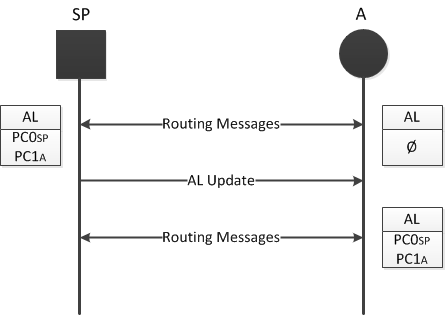
\includegraphics[width=0.5\textwidth]{images/node_states_authorized.png}
%  	\caption{Normal operation between a \acf{SP} and an unauthenticated node
%  	(A)including an \ac{AL} Update message.}
%	\label{fig:node_states_authorized}
%\end{figure}

When a node has been issed a \ac{PC} and become a trusted node in the network,
it is almost ready to take part in the sending and forwarding of routing
announcements. But before a node can take part in the routing in the network, it
has to be able to append one-time-passwords to its routing announcements, and to
verify other nodes' one-time-passwords as it receives routing announcements from
them.

\subsection{Keystream generation}
The \acp{OTP} are actually smaller extracts of larger keystreams shared
between direct neighbors in the network. When a node started its routing
protocol daemon and before discovering the \ac{SP} in the previous step, it
generates a high entropy pseudo-random master key and a regular pseudo-random
\ac{IV}. The master key needs high entropy to be as random as possible, because
the security of this design relies on this key to both be secret and not
guessable.

When the node is ready to share its keystream for the first time, the node will
generate a new ephemeral key by encrypting $K_{ephemeral} =
E_{K_{master}}\{i\}$ where $i = 1,2,3\ldots$ and a corresponding \ac{IV}
generated in the same manner as the previous \ac{IV} for the master key. In
addition, a large nonce is generated with a pseudo-random function, also in the
same pseudo-random fashion as the \acp{IV}. To elaborate, this pseudo-randomness
does not need strong randomness with a high entropy like the master key, it only
needs to be (with high probability) different for each time.

With the current ephemeral key, generated with $i = 1$, \ac{IV} and nonce, the
node can now generate its first keystream to be used as \acp{OTP} for its
routing announcements. The keystream is generated by encrypting the nonce with
the ephemeral key multiple times, each time extending the size of the
keystream. Each encryption is a full ``Cipher-block chaining'' AES encryption,
i.e. each encryption step referred to here (and later) are actually multiple
encryptions using the AES-CBC mode.

In the first encryption (full AES-CBC) the supplied \ac{IV} is used, while in
the next iterations a 16 byte extract of the output from the previous encryption
(ciphertext) is used as \ac{IV}. To explain, this is basically a \ac{CBC} mode
encryption of multiple AES-CBC blocks. Figure \ref{fig:keystream_generation}
shows the process assuming the ephemeral key, IV and nonce have already been
created.

\begin{figure}[h]
	\centering
  	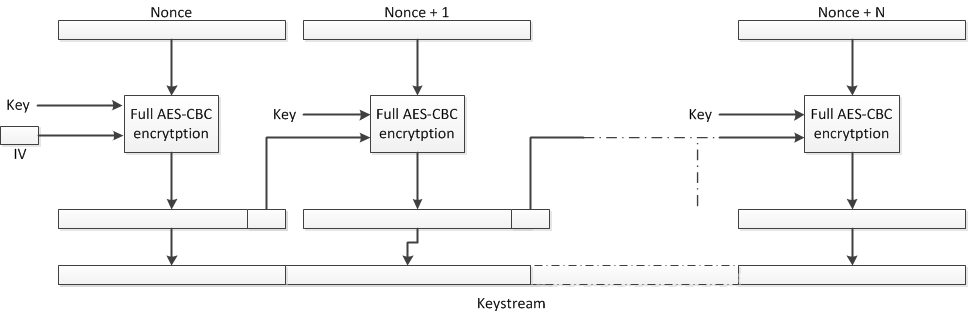
\includegraphics[width=\textwidth]{images/keystream_generation.png}
  	\caption{Keystream generation based on the supplied Nonce, Key and IV.}
	\label{fig:keystream_generation}
\end{figure}

In the figure there are some boxes marked with ``Full AES-CBC encryption''. This
is meant to illustrate that within each of those boxes there is a full AES-CBC
encryption taking place, with multiple steps according to the standards of
AES-CBC. The reader should also notice that as the ciphertext output of each of
those boxes are much larger than the AES block size, therefore only an AES block
size extract at the end of the ciphertext is used as an \ac{IV} for the next
encryption step, instead of the whole ciphertext which would usually be done in
CBC as there the ciphertext corresponds to the correct block size.

The lifetime of a node's keystream is determined by two factors. First, the
keystream is updated at a regular time interval (60 seconds is used in this
thesis' implementation). Second, the keystream could be exhausted before this
time interval. For whichever comes first, a new keystream has to be generated,
and shared with all direct neighbors. Each time a new keystream-material message
is created, the ephemeral key is generated by increasing the plaintext 'i'. I.e.
the second time a keystream is generated, the ephemeral key is
$E_{K_{master}}\{2\}$.

\subsubsection*{Keystream Sharing}
Now, before this keystream can be used to authenticate routing announcements,
the node will have to share the keystream with its direct neighbors. This is
done by sending all the material necessary for the neighbor to create the
keystream themselves and signing the message with your private key. I.e. the
node will have to send the ephemeral key, \ac{IV} and nonce to its neighbor.
Here it is crucial that the key stays secret between the neighbors, therefore
the node will have to encrypt the ephemeral key with its neighbors' public keys
and send a unicast message with the keystream material to each one of them. The
details around sharing the keystreams will be further explained in the
following section regarding all messages sent in the network
(\ref{sect:am_messages}).

\subsection{Using \acfp{OTP} from Keystream}
Once the keystream has been shared with the neighbors, the node will begin to
extract smaller chuncks of the keystream and use an \ac{OTP} for each
routing announcement it generates itself, or forwards from other trusted
neighbors. In addition to the \acp{OTP} appended to the announcements,
the node keeps a counter, or sequence number, to keep track of which
\ac{OTP} it has used in order not to use the password twice.

Similarily the node will have to both verify the correctness of the \acp{OTP}
received in announcements from its trusted neighbors, and that they have not
been received before. If the password has been received before the annoucement
needs to be dropped, and assumed to be part of a replay-attack. If the node
would have accepted re-using of one-time-passwords, an attacker could listen
and record valid one-time-passwords and re-use them with false routing
information in order to disrupt the routing in the network.

How to check for replayed one-time-passwords is further elaborated in the next
chapter, but simply put - a sliding window recording the last announcements are
used, setting a bit value to true if an announcement with the corresponding
sequence number (keystream sequence number, not from original protocol) has been
received, and zero if not.

\subsection{Discovering New Neighbors}
Up until this point, the node only had only discovered the \ac{SP} and after the
authentication handshake shared their keystream material in order to be able to
trust each others' routing annoucements. Because of the trust mode being used in
this design, each routing annoucement from the \ac{SP} are trusted, even if they
are re-broadcasts (forwarded by the SP) originating from other nodes not yet
known to the new node. This means that the routing table of our node could
possibly fill up with unknown nodes, reachable through \ac{SP}. To have all
data streams go through the \ac{SP} however, would be less than ideal. If some
of those nodes are direct neighbors of our node, they should be able to
communicate directly.

Therefore a discovery mode of other trusted (by the network at least) nodes
needs to be handled. Until now, if you received any routing announcements
from an unknown neighbor you would have dropped the packet. After becoming an
authenticated node, the node will now instead engage in a exchange of \acp{PC}
with the other neighbor. If the neighbor sends you a \ac{PC} with a signature
of the \ac{SP} which you are able to verify, you will add the node to your
\ac{AL} and send him your \ac{PC} - if you have not sent it already.

The verification of the ownership of the \ac{PC} is not performed before
receiving the keystream-material message which occurs soon after sharing
\acp{PC}. As a remainder the keystream-material message is signed with the
private key of the sender. Therefore, assuming the nodes has not been
compromized, the ownership of the neighbors are verified by checking the
validity of said signatures.

\section{Detailed Entity Description}
\label{sect:detailed_ent}
\subsection{\acf{PC}}
\label{subsect:detailed_pc_descr}
In a scenario where actors try to communicate with each other, without the
Internet or other communication infrastructure available one cannot depend on a
\ac{PKI} for authentication of the actors. One needs the option of being able
to verify actors physically (out-of-band) and then issuing them an
authentication token to be used during this scenario. This is where the
\aclp{PC} comes in handy. Regular \acp{EEC} should not be used for issuing new
certificates, per RFC2459 \cite{rfc2459}, and even if one did use them for
this purpose there is no definition on how to handle topics as path validation
and such.

Using \acp{PC} this issue can be handled in a well-defined manner. The field
``pCPathLenConstraint'' is used for constraining the depth of the certificate
chain below the \ac{PC} itself. I.e. if a \ac{PC} has a pCPathLenConstraint of
zero, the \ac{PC} cannot issue any other \acp{PC} itself, while if the 
pCPathLenConstraint value is one the \ac{PC} can be used to issue new \acp{PC}
which again will have a pCPathLenConstraint of zero, and so on.

For our scenario, the pCPathLenConstraint value should never exceed one, or else
it will once again be difficult to handle path validations. Every node trying to
verify a \ac{PC} need to know the issuer of the certificate directly, and not
indirectly through root \acp{CA} as is possible if you have a \ac{PKI}.

A \ac{PC} is almost a regular certificate, except for some values that are
forbidden to use, some values that are required to use, and some values that
must be used in a well defined way \cite{rfc3820}. Below are the
fields that are included in this system design:
\begin{itemize}
  \item Subject Name: $<$Isser Name$>$ + ``CN: $<$SHA-1(Public Key)$>$''
  \item Issuer Name: $<$Subject Name of Issuer$>$
  \item Serial Number: ``$<$SHA-1(Public Key)$>$''
  \item X509v3 Extensions:
  \begin{itemize}
    \item Key Usage: ``Digital signature, Key encipherment''
    \item ProxyCertInfo:
    \begin{itemize}
      \item pCPathLenConstraint: $<$0 or 1$>$
      \item proxyPolicy: 
      \begin{itemize}
        \item policyLanguage: ``id-ppl-anyLanguage''
        \item policy: ``Role:$<$sp or authenticated$>$,Routing:$<$full or limited$>$,Application:$<$full or limited$>$''
      \end{itemize}
    \end{itemize}
  \end{itemize}
\end{itemize}
Per RFC3820 \cite{rfc3820} the subject name has the constraint that it
``should be unique amongst all Proxy Certificates issued by a particular Proxy
Issuer''. The modal verb ``should'' used in this requirement is used in order
to ease this requirement so that a method creating a unique name with a high
probability, but not provable uniqueness, can be accepted. Therefore using a
SHA-1 digest of the public key used by the node is regarded as ``good enough'',
or ``unique enough''.

The same requirement is true for the serial number, and allows the serial number
to be the same as the subject name except for the ``CN:'' prefix.

The specifications requires the ``Digital signatures'' value for the ``Key
Usage'' extension because a \ac{PC} can be used to sign the keystream material
messages. ``Key encipherment'' is also necessary in this extension because other
neighbors need to use your public key to encrypt their ephemeral keys when they
want to share their keystream with you.

The ``policyLanguage'' field is set to the default value, leaving the
language used in the policy field later to be handled correctly by the
application, rather than being universally understandable.

Finally, the last field called ``policy'' might be of greates interest. This
field explains what rights the given \ac{PC} has for this design. Three values
have been defined for use in this design:

\begin{itemize}
  \item Role - Node's role in the network
  \item Routing - Whether the node can partake in the routing
  \item Application - Whether the node has access to the application layer
\end{itemize}

These values are specific to this design, and might not be desired in
other applications. The first value, ``role'', is used to declare which role the
node has been given. It can be ``sp'' which means the node as administrative
rights in the network, or ``authenticated'' meaning the node is trusted by the
\ac{SP} and should be trusted by all other nodes in the network.

The ``routing'' value can be ``full'' or ``limited''. If it is full the node is
able to generate and broadcast its own routing announcements, and forward its
trusted nodes' routing annoucements. This means the node partakes completely in
the network and might be placed in a path between two nodes in the network. The
``limited'' value is used so a node can become an end-node, but not a node in a
path between other nodes. I.e., it can send its own routing announcements, but
it cannot forward other nodes' routing annoucements. If a node with limited
rights does forward other nodes' announcements they must be dropped. In
addition, a detection system of misbehaving nodes should pick up this as
potentially malicious behaviour, but this is not being implemented as
previously explained in Limitations (\ref{limit:malicious_behaviour}).

The last value, ``application'', is used to declare whether the node should have
access to the upper layers and being able to use the applications running on top
of the \ac{MANET}. This restriction is useful if one has special devices in the
field only used to route/forward packets in the network, acting similar to
routers in the regular Internet, but not being able to e.g. respond to
application requests. Nodes which do not use the application layer will reside
in each nodes' routing tables, but should not show up as available nodes on the
upper layers.

\subsubsection*{\acf{PC0}}
A \acl{SP}'s \ac{PC0} would typically be filled with the values in the
\ref{tab:pc0_values}. For illustration, this \ac{PC} has been issued by the
\ac{SP}'s regular \ac{LLPKC} issued by NTNU.
\begin{table}[h]
	\begin{tabularx}{\linewidth}{ | l | X |}
		\hline
 		\textbf{X.509 Field} & \textbf{Value}\\\hline
		Subject Name & C=NO, L=Trondheim, O=NTNU, OU=ITEM, CN=Espen, CN=$<$SHA-1(Public Key)$>$ \\\hline
		Issuer Name & C=NO, L=Trondheim, O=NTNU, OU=ITEM, CN=Espen \\\hline 
		Serial Number & $<$SHA-1(Public Key)$>$ \\\hline 
		Key Usage & Digital signature, Key encipherment \\\hline 
		pCPathLenConstraint & 1 \\\hline 
		policyLanguage & id-ppl-anyLanguage \\\hline 
		policy & Role:sp,Routing:full,Application:full \\\hline 
	\end{tabularx}
	\caption{Values in \acf{PC0}}
	\label{tab:pc0_values}
\end{table}
The zero in the PC0 abbreviation is used to indicate that the certificate is at
a depth of zero and has a pCPathLenConstraint of one, meaning that the \ac{SP}
is allowed to issue new \acp{PC}, but that the children of the \ac{PC0} cannot
be used to issue new \acp{PC} again.

\subsubsection*{\acf{PC1}}
If the PC0 above was used to issue a regular PC1 to an authenticated node, the
values might look like the ones in Table \ref{tab:pc1_values}.
\begin{table}[h]
	\begin{tabularx}{\linewidth}{ | l | X |}\hline
 		\textbf{X.509 Field} & \textbf{Value}\\\hline
		Subject Name & C=NO, L=Trondheim, O=NTNU, OU=ITEM, CN=Espen, CN=$<$SHA-1(PubKey(SP))$>$, CN=$<$SHA-1(Public Key)$>$ \\\hline
		Issuer Name & C=NO, L=Trondheim, O=NTNU, OU=ITEM, CN=Espen, CN=$<$SHA-1(PubKey(SP))$>$ \\\hline
		Serial Number & $<$SHA-1(Public Key)$>$ \\\hline 
		Key Usage & Digital signature, Key encipherment \\\hline 
		pCPathLenConstraint & 0 \\\hline 
		policyLanguage & id-ppl-anyLanguage \\\hline 
		policy & Role:authenticated,Routing:full,Application:full \\\hline 
	\end{tabularx}
	\caption{Values in \acf{PC1} if issued by the \ac{PC0} above.}
	\label{tab:pc1_values}
\end{table}
The interesting part here is too see that the subject name contains the full
subject name of the issuer in addition to the hash value of the public key used
in the PC1. Note also that the pCPathLenConstraint now denies the owner to issue
other acp{PC} using this certificate.

\subsection{\acf{SP}}
The term \acl{SP} was coined by Dr. Lawrie Brown \cite{lawrie:technotes}.
\acp{SP} are used in place of regular \acp{CA} for \acp{PC}. The \ac{SP}
determines whether a node should be issued a \ac{PC} and if so which policies to
attach. The \ac{SP} drastically distinguishes itself from regular \acp{CA}
because it breaks the hierarchical model usually associated with \acp{CA} when
they are part of a \ac{PKI}.

A \ac{SP} can also be part of a \ac{PKI} (issued a regular public key
certificate), but because of our scenario, it can be difficult or impossible to
verify its regular certificate. Therefore, this verification is handled
out-of-band instead.

In this design, the \ac{SP} is a master node which decides which nodes can get
access to the network and if so what rights they have. The \ac{SP} assigns its
\ac{PC0} with all the rights which might be useful for the current scenario, so
that it can delegate those rights to other nodes when issuing them \acp{PC1}. In
a larger network, there would typically be more than one \ac{SP}

\subsection{\acf{AL}}
The \ac{AL} is a local list that each trusted node including the \ac{SP} in
the network maintain to keep track of which nodes they knows and the necessary
information about them. An \acl{AL} stores these values for each node they have
met and shared their \acp{PC} with:
\begin{table}[h]
	\centering
	\begin{tabular}{| l |}\hline
 		\textbf{\acl{AL}}\\\hline
		ID\\\hline
		Address \\\hline
		Role \\\hline 
		Subject Name \\\hline 
		Public Key \\\hline  
	\end{tabular}
	\caption{\acf{AL} content}
	\label{tab:al_content}
\end{table}
Both the ``ID'' and ``Subject Name'' fields stored for each node are unique, so
one could ask why one needs the ID field when the unique subject name is used in
accordance with RFC3820 (\cite{rfc3820}). The answer is actually quite simple,
it is easier and safer to look for the ID value when going searching in the
\ac{AL} because it is a number while the subject name value is a text.

For all nodes but the \ac{SP} in the network, the first entry in the \ac{AL} is
the \ac{SP}. This is only natural because the \ac{SP} is the first node they
start to trust as it is the one node that actually issued their \ac{PC} in the
first place. To illustrate this, if you go back to the two nodes' \acp{PC} in
Tables \ref{tab:pc0_values} and \ref{tab:pc1_values} and you have a third node
with these two nodes in its \ac{AL}, the \ac{AL} might look like Table
\ref{tab:al_content_3_nodes}.
\begin{table}[h]
	\centering
	\begin{tabularx}{\linewidth}{| l | X |}\hline
 		\textbf{Fields} & \textbf{Values}\\\hline
 		\hline
		ID & 45251\\\hline
		Address & 192.168.57.1\\\hline
		Role & SP\\\hline 
		Subject Name & C=NO, L=Trondheim, O=NTNU, OU=ITEM, CN=Espen, CN=$<$SHA-1(2AF2E5C75C\ldots)$>$\\\hline
		Public Key & 2AF2E5C75C\ldots\\\hline
		\hline
		ID & 1341\\\hline
		Address & 192.168.57.45\\\hline
		Role & Authenticated\\\hline 
		Subject Name & C=NO, L=Trondheim, O=NTNU, OU=ITEM, CN=Espen, CN=$<$SHA-1(2AF2E5C75C\ldots)$>$, CN=$<$SHA-1(DA912BC9F5\ldots)$>$\\\hline
		Public Key & DA912BC9F5\ldots\\\hline  
	\end{tabularx}
	\caption{An \acf{AL} in a network with three trusted nodes.}
	\label{tab:al_content_3_nodes}
\end{table}
Note that the arbitrarily chosen values for e.g. the Public Key here does not
show a complete size public key. Also, the public keys stored in the \ac{AL}
would be stored as their real binary values, and not Base64-encoded as the table
portrays. In the subject name there is a common name part with ``SHA-1()'' -
meaning that the content here would actually be the sha-1 digest of the content
inside the brackets.

\subsection{\acf{NL}}
The \acl{NL} is a list each node in the network maintains to keep track of its
current neighbors and the necessary information about them.
\begin{table}[h]
	\centering
	\begin{tabular}{| l |}\hline
 		\textbf{\acl{NL}}\\\hline
		ID\\\hline
		Address\\\hline
		Sliding window\\\hline 
		Last sequence number\\\hline 
		Keystream\\\hline
		Number of wrong OTPs\\\hline
		Time keystream received\\\hline
	\end{tabular}
	\caption{\acf{NL} content}
	\label{tab:nl_content}
\end{table}
Table \ref{tab:nl_content} shows the content fields for each entry in the
\ac{NL}. The first important thing to recognize is that the node entries in the
\ac{NL} are not necessarily the same as the node entries in the \ac{AL}. When a
node meets new neighbors and looses old direct neighbors (which are still in
the network nevertheless) new entries are added while old entries are removed.
This means also that the index in the two lists are not the same - and here's
where the use of the ID field comes in. Whenever both lists has to be looked up,
the ID field is used in order to retrieve the same node from both lists.

Besides the ID and the address the keystream field should be expected to reside
in the \ac{NL} by the observant reader. If not, this is where the keystreams of
your neighbors are stored, and updated each time you receive a new
keystream-material message from said neighbor. There are four other fields too
however, which might not be expected by the reader. These fields play an
important part in mainstaining this list and most importantly - replay attack
protection.

First, the ``Time keystream received'' field stores the time (in seconds) when
the last keystream from this neighbor was received. The \acl{AM} regularly
checks to see if it has not received keystreams from nodes in the \ac{NL} for
some time, and purges all entries older than a defined timeframe. This is mainly
to keep the \ac{NL} up to date and short, as the keystreams take up memory
storage.

The remaining three fields are quite more interesting, as they are used for
replay attack protection.

\subsubsection*{Sliding Window}
The sliding window is a bit array of 64 bits size \cite{peterson2007computer}.
This window is used in order to decide whether a routing announcement should be
allowed through to the routing protocol, or if the \ac{AM} should block and
drop the announcement. Each bit in the window can either be 0 or 1, and it is
used to declare whether an \acf{OTP} already has been received (bit set to 1)
or not (bit set to 0).

The ``last sequence number'' field is used to indicate the last, or highest,
keystream sequence number of the last routing announcement received from this
neighbor. If the last sequence number is X, then the sliding window corresponds
to the the sequence numbers between X-63 and X. I.e. the sliding window shows
whether an \ac{OTP} from this range has been received or not.

For a node to accept a routing annoucement from a direct neighbor (which is in
its \ac{NL}), the following MUST be true:
\begin{itemize}
  \item the \ac{OTP} sequence number must either be inside the sliding window,
  	or higher than the current last sequence number, and
  \item the same sequence number must not have been received before, i.e. the
  	bit at its sliding window position must be 0, and
  \item the \ac{OTP} must match the keystream at this sequence number offset.
\end{itemize}
Note that when a new keystream is calculated for a neighbor, the old sliding
window and last sequence number are replaced so the same sequence numbers can be
used again.

The last field, ``Number of wrong OTPs'', is increased whenever a received
routing announcement fails the checks above, i.e. if its an too old sequence
number, it has been received before, or if the \ac{OTP} does not match the
expected \ac{OTP} from the keystream. If this value is too high, the node will
delete the neighbor entry from its \ac{NL} and request a new keystream-material
message. This value is reset to zero when a routing announcement from the same
neighbor pass all the checks above, assuming the problem has been fixed.

\section{Authentication Module Messages}
\label{sect:am_messages}
This section describes the different messages sent within, or modified by, the
\ac{AM} extension. This includes how they are created, what payload they
contain, if and how the information is secured from malicious actors, and
finally to whom and how often they are sent during normal operation.

Each \ac{AM} message has a header field which declares what kind of message
follows in the payload and the unique ID of the sender. Some messages contain
the exact same payload, but might have different message identifiers because the
message can be sent by different purposes.

\subsection{Node Discovery}
Node discovery is not actually a part of the \ac{AM} itself, but it is the
main event that triggers the \ac{AM} and is described here to make the context
more clear to the reader.

Whenever a trusted node receives a routing announcement containing an \acf{OTP}
from a new neighbor, i.e. a node which is not in the \acf{NL}, the trusted node
needs to check the \acf{AL} to see if the node is a trusted node. If the node
can be found in the \ac{AL} the trusted node will request and send its
keystream-material message.

If the neighbor is not found in the \ac{AL} however, the node will send its
\ac{PC} and request the neighbor's \ac{PC}. In addition, both nodes will after
verifying the other nodes' \ac{PC} send its keystream-material to the other.

If the routing announcement does not contain an \ac{OTP} at all, meaning the
neighbor is either a new or untrusted, regular authenticated nodes will ignore
and drop it as they do not take part in the authentication of new nodes. If the
trusted node is also the \acf{SP} however, it will invite the unknown neighbor
to an authentication handshake before dropping the packet.

\subsection{Authentication Handshake}
The authentication handshake describes which messages are sent while
authenticating a new node to the network. If the handshake is successful the two
nodes participating in the handshake will share their keystream-materials with
one another.

\subsubsection*{Handshake Invite}
The handshake invite message is a rather simple message. Its header declares
that it is an ``invite message'', and the payload only contains the SP's 
\ac{PC}. The \ac{PC} is sent in the beginning in order for the new node to be
able to verify the certificate before engaging in the handshake.

\subsubsection*{\acl{PC} Request}
This message contains the field declaring it is a ``certificate request
message'' and its payload contains a X.509\_REQ data structure
\cite{viega2002network}. This data is essentially a certificate without an
issuer's signature, containing all the values it wishes the \ac{SP} to grant
it.

The request data structure also contains the extensions being used, and
specifically the sender will request certain rights through the policy field of
the proxy certificate. E.g. it can request full routing and full application
rights as mentioned in Section \ref{subsect:detailed_pc_descr}.

\subsubsection*{\acf{PC} Issue}
Completing the handshake is a message containing the signed certificate. If the
\ac{SP} was able to verify the new node's public key, the \ac{SP} would sign the
request in addition to adding some values, possibly changing some of the
requested values, and sending it all in one message.

After this message, the \ac{SP} waits for the first keystream-material message
from the newly authenticated node as an acknowledgement from the recipient,
after which the \ac{SP} sends its keystream-material to the new node as well.

\subsection{Keystream-Material Message}
This message contains two headers - a regular AM header declaring the type of
message and ID of the sender, and a special header declaring the different
lengths of the contents in the payload.

The payload contains everything needed to create the sender's keystream, i.e. a
nonce, an ephemeral key encrypted with the recipients public key, an IV, and a
digital signature. The signature is used tp prove the authenticity of the
message, i.e. to prove the integrity of the message content and to authenticate
the sender - or prove the sender is who is claims to be. The digital signature
is created by creating a message digest of the nonce, IV, and unencrypted (!)
ephemeral key and encrypting the message digest with the senders private key.

TODO: FIGURE OF THE PACKET HERE!

As can be seen in the figure above, the encrypted ephemeral key is appended at
the end. This, and the decision to make the digital signature from the
unencrypted key, is done in order to make the packet ``re-usable'' - remember
this packet has to be sent by the creator to each of its neighbors, and with
this design only the ephemeral key needs to be encrypted and appended to the
``standard'' packet for each recipient. This not only makes the design easier,
it saves overhead by not having to create a digital signature for each recipient
of the packet.

This message is sent to all neighbors periodically (changing the keystream), or
when the keystream has been exhausted - whichever comes first.

\subsubsection*{Keystream-Material Request}
There is a special case the keystream-material sharing. If a node continuously
receives routing announcements with bad \acp{OTP}, the node will assume the
neighbor has created a new keystream but its keystream-material message has not
been successfully received by this node. Because this often happens if the
packet delivery ratio is low, the node also assumes that the other neighbor does
not have its keystream-material.

The node therefore generates a regular keystream-material message, only
different by the first header type declaring this to be a ``keystream request'',
and sends it to its neighbor as if it was a new neighbor. Note that no new
keystream-material is created here, it is only a ``re-sending'' of the old
packet appended with the current ephemeral key (encrypted).

\subsection{Modified Routing Announcements}
The routing announcements are sent by the original routing protocol and not by
the \ac{AM}, but a small but significant alteration to the routing protocol has
to be made in order to append the \acp{OTP} to the routing announcements.
Therefore this will be discussed here briefly.

The routing announcements are appended with 16 bits extracts from the keystream,
called one-time-passwords. Additionally, each routing announcement is also
appended with a sequence number for which the offset of the keystream the
\ac{OTP} matches.

TODO: Add figure showing these messages, and explicitly the 16 bits extracted
from the keystream\ldots

For each routing announcement a neighbor receives, it checks the \ac{OTP} at the
given offset of the senders keystream and if it matches - it assumes the message
is from its trusted neighbor. If the \ac{OTP} does not match the packet will be
dropped as discussed earlier.

%\begin{figure}[h]
%	\centering
%  	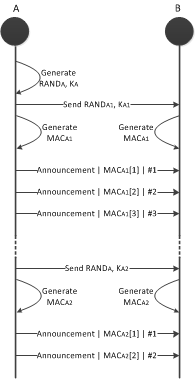
\includegraphics{images/mac_ogm_msc.png}
%  	\caption{Node A peridically generates a new pseudo-random value and a
%  	corresponding symmetric key which it shares with its neighbor B. Node A use
%  	an extract of a generated MAC of this value in each of its routing
%  	announcements hereafter.}
%	\label{fig:mac_ogm_msc}
%\end{figure}

